\documentclass{beamer}
\usepackage[utf8]{inputenc}
\usepackage[T1]{fontenc}
\usepackage{amsmath,amssymb}
\usepackage{graphicx}
\usepackage{booktabs}
\usepackage{tabularx}
\usepackage{tikz}
\usetikzlibrary{arrows.meta, shapes.geometric, positioning}
\usepackage{multirow}
\usepackage{xcolor}

\usetheme{Madrid}
\graphicspath{{images/}}

\hypersetup{unicode=true,
  pdftitle={HBCC: Hybrid Binarized Context Cluster},
  pdfauthor={Nguyen Viet Hung, Nguyen Ba Nam}}

\title[HBCC]{HBCC: Hybrid Binarized Context Cluster\\for Lightweight Image Classification}
\subtitle{Research Presentation}
\author[Hung \& Nam]{Nguy\~{\^e}n Vi\d{\^e}t H\`ung \quad \& \quad Nguy\~{\^e}n B\'a Nam}
\institute[HCMUS]{University of Science, VNU--Ho Chi Minh City (HCMUS)\\[4pt]
  \small Supervisor: Prof.\ L\^e Ho\`ang Th\'ai}
\date{July 2026}

\begin{document}

% ============================================================
% Slide 1: Title
% ============================================================
\begin{frame}
  \titlepage
\end{frame}

% ============================================================
% Slide 2: Outline
% ============================================================
\begin{frame}{Outline}
  \tableofcontents
\end{frame}

\section{Problem \& Motivation}

% ============================================================
% Slide 3: Problem Statement
% ============================================================
\begin{frame}{Problem Statement}
  \begin{block}{Goal}
    Build a \textbf{lightweight} image classifier that is accurate
    and efficient for resource-limited settings.
  \end{block}

  \vspace{0.3em}
  \textbf{The core tension:}
  \begin{itemize}\setlength\itemsep{5pt}
    \item \textbf{Heavy models} (ResNet-18, 11M params):
          accurate but far too expensive.
    \item \textbf{Lightweight CNNs} (MobileNet, ShuffleNet):
          efficient, but accuracy drops to $\sim\!91\%$.
    \item \textbf{Clustering models} (CoC):
          global context but loses local texture $\to$ only 88\%.
  \end{itemize}

  \vspace{0.2em}
  \begin{alertblock}{Research Question}
    Can combining local convolution with global clustering
    outperform each approach alone, at the same parameter budget?
  \end{alertblock}
\end{frame}

% ============================================================
% Slide 4: Motivation
% ============================================================
\begin{frame}{Why HBCC? --- Existing Method Gaps}
  \begin{block}{Observation}
    No single lightweight method handles both local texture and
    global context. HBCC is designed to bridge this gap.
  \end{block}

  \vspace{0.5em}
  \begin{tabular}{lp{3.0cm}p{3.6cm}}
    \toprule
    \textbf{Method} & \textbf{Strength} & \textbf{Key Weakness} \\
    \midrule
    ResNet-18     & Strong local features      & 11M params --- too heavy \\[4pt]
    MobileNetV2   & Efficient depthwise conv   & Misses long-range context \\[4pt]
    ShuffleNetV2  & Efficient channel shuffle  & Misses global context \\[4pt]
    CoC           & Global clustering, $O(NM)$ & Loses local texture \& edges \\[4pt]
    \textbf{HBCC} & \textbf{Local + global}    & Latency overhead (clustering ops) \\
    \bottomrule
  \end{tabular}
\end{frame}

\section{Datasets}

% ============================================================
% Slide 5: Datasets
% ============================================================
\begin{frame}{Datasets: CIFAR-10 \& CIFAR-100}
  \begin{columns}[T]
    \begin{column}{0.54\textwidth}
      \textbf{Why CIFAR-10 \& CIFAR-100?}
      \begin{itemize}\setlength\itemsep{6pt}
        \item \textbf{Small images} ($32\!\times\!32$) match HBCC's design:
              all 4 stages preserve and process the full spatial content.
        \item \textbf{Standard benchmarks}: fair, reproducible comparison
              with all baselines.
        \item \textbf{Fast iteration}: 60\,000 images allow rapid
              ablation across many architecture variants.
        \item \textbf{Two difficulty levels}: 10 vs.\ 100 classes,
              same architecture, same training setup.
      \end{itemize}
    \end{column}
    \begin{column}{0.42\textwidth}
      \begin{block}{Dataset Summary}
        \centering
        \begin{tabular}{lcc}
          \toprule
                     & \textbf{C-10} & \textbf{C-100} \\
          \midrule
          Classes    & 10   & 100  \\
          Train      & 45K  & 45K  \\
          Val        & 5K   & 5K   \\
          Test       & 10K  & 10K  \\
          Resolution & \multicolumn{2}{c}{$32\!\times\!32$} \\
          \bottomrule
        \end{tabular}
      \end{block}

      \vspace{0.4em}
      \textbf{Known Limitations:}
      \begin{itemize}\small\setlength\itemsep{4pt}
        \item Low resolution --- not real-world imagery.
        \item No ImageNet validation yet.
        \item Baselines use weaker augmentation than HBCC.
      \end{itemize}
    \end{column}
  \end{columns}
\end{frame}

\section{HBCC Methodology}

% ============================================================
% Slide 6: Context Cluster (CoC)
% ============================================================
\begin{frame}{Foundation: Context Cluster (CoC)}
  \begin{block}{Key idea}
    Treat the image as a \textbf{set of points}, group similar ones ---
    no $O(n^2)$ attention matrix needed.
  \end{block}

  \vspace{0.15em}
  \begin{columns}[T]
    \begin{column}{0.53\textwidth}
      \begin{enumerate}\setlength\itemsep{3pt}
        \item \textbf{Represent:} each pixel as a 5D point
              $(R, G, B, x, y)$ --- color + normalized position.
        \item \textbf{Derive} cluster centers via adaptive avg-pooling.
        \item \textbf{Assign} each point to its nearest center
              by cosine similarity.
        \item \textbf{Aggregate} cluster-mate features,
              then \textbf{dispatch} back to spatial positions.
      \end{enumerate}
    \end{column}
    \begin{column}{0.42\textwidth}
      \centering
      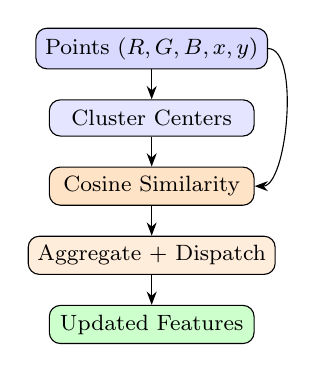
\begin{tikzpicture}[>=Stealth, node distance=0.38cm,
          every node/.style={font=\footnotesize, align=center},
          box/.style={draw, rounded corners, minimum width=2.6cm,
                      minimum height=0.46cm}]
        \node[box, fill=blue!15]    (pts)  {Points $(R,G,B,x,y)$};
        \node[box, fill=blue!10,   below=of pts]  (ctr)  {Cluster Centers};
        \node[box, fill=orange!22, below=of ctr]  (sim)  {Cosine Similarity};
        \node[box, fill=orange!14, below=of sim]  (agg)  {Aggregate + Dispatch};
        \node[box, fill=green!20,  below=of agg]  (out)  {Updated Features};
        \draw[->] (pts) -- (ctr);
        \draw[->] (ctr) -- (sim);
        \draw[->] (pts.east) to[out=0,in=0,looseness=0.6] (sim.east);
        \draw[->] (sim) -- (agg);
        \draw[->] (agg) -- (out);
      \end{tikzpicture}
    \end{column}
  \end{columns}
\end{frame}

% ============================================================
% Slide 7: Hybrid Block
% ============================================================
\begin{frame}{Hybrid Block: Local + Global in Parallel}
  \begin{columns}[T]
    \begin{column}{0.43\textwidth}
      \centering
      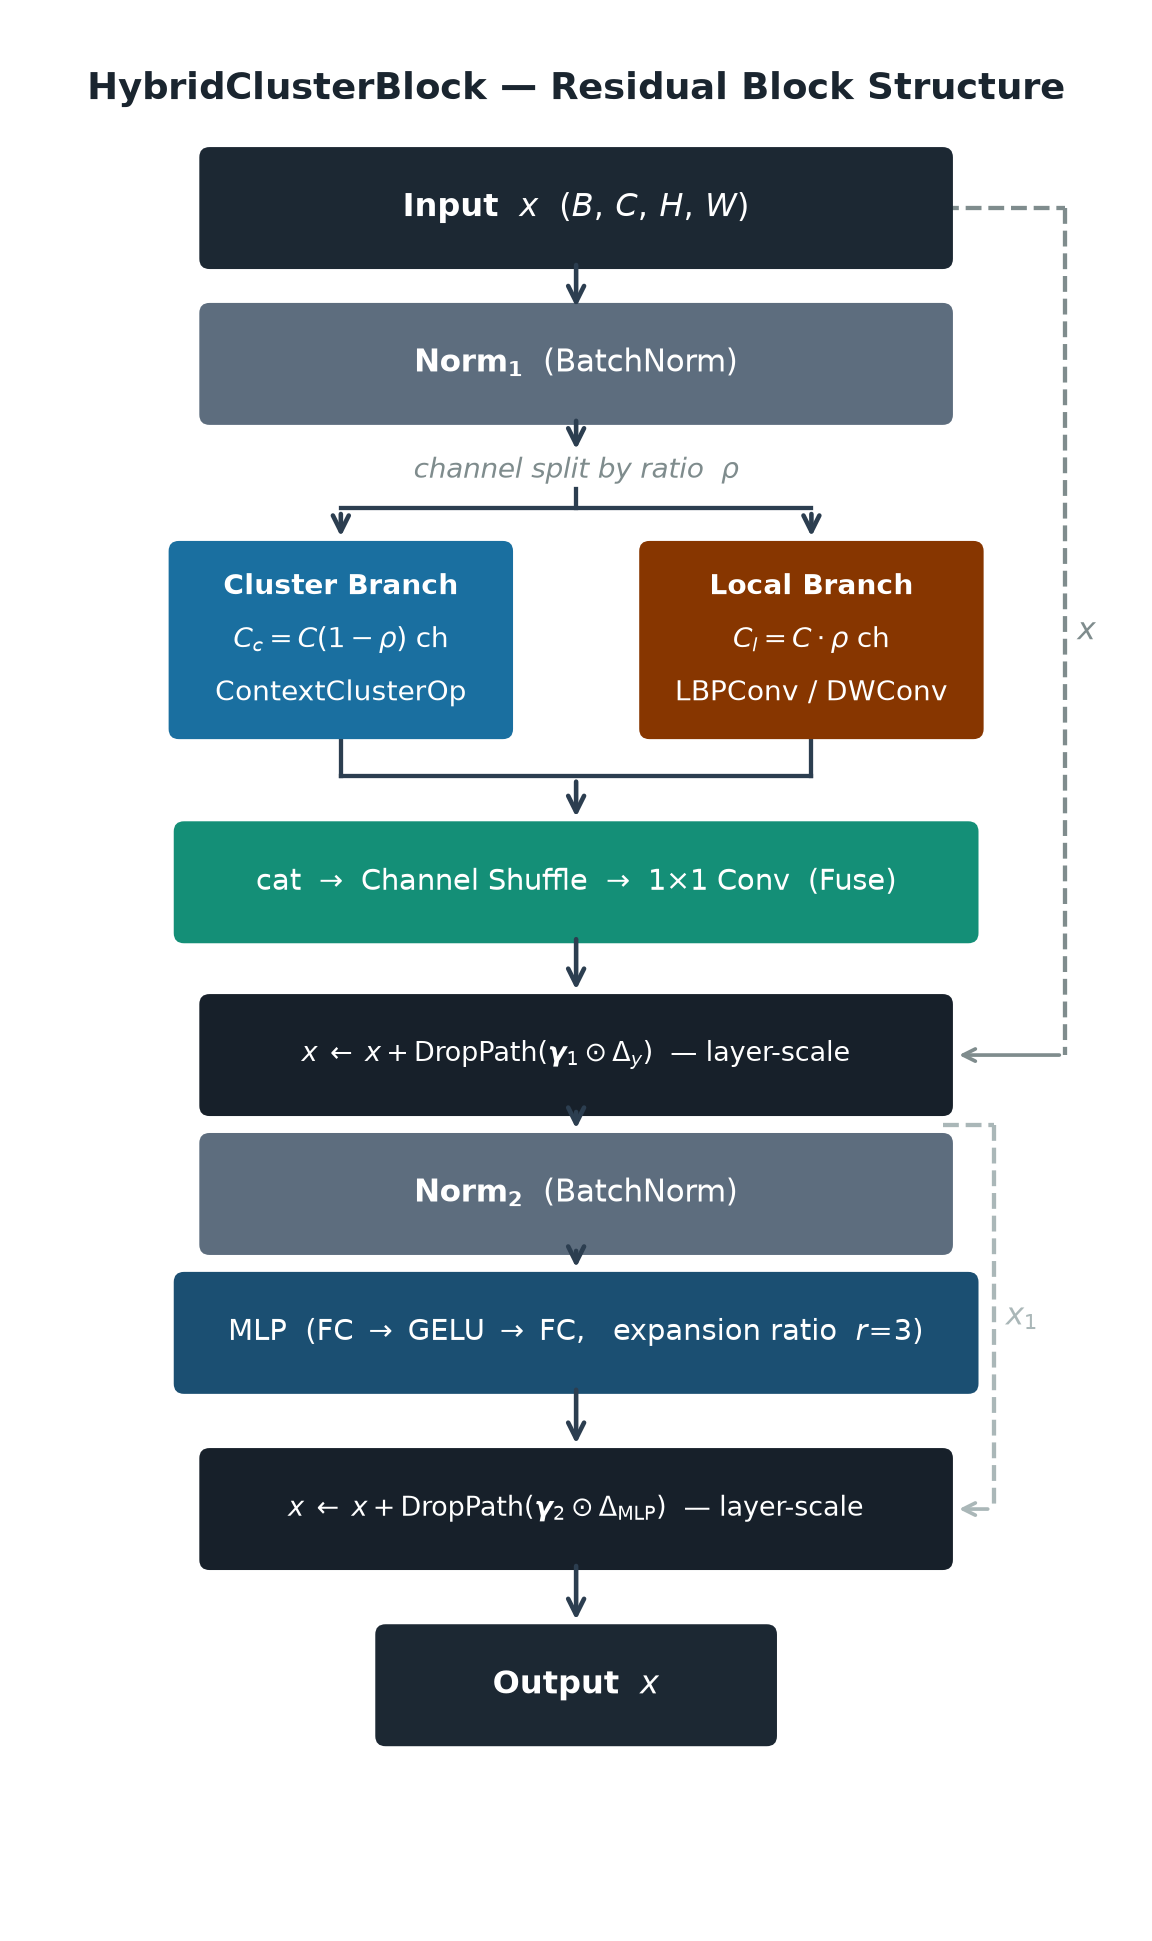
\includegraphics[width=\textwidth,
                       height=0.73\textheight,
                       keepaspectratio]{fig_hybrid_block}
    \end{column}
    \begin{column}{0.53\textwidth}
      \vspace{0.3em}
      \textbf{Channel split by ratio $\rho$:}
      \begin{itemize}\small\setlength\itemsep{5pt}
        \item \textit{Local branch} ($\rho C$ ch):\\
              LBPConv (Stage 1) or DWConv (Stage 2).
        \item \textit{Cluster branch} ($(1{-}\rho)C$ ch):\\
              Context Cluster (CoC).
      \end{itemize}

      \vspace{0.4em}
      \textbf{After the branches:}
      \begin{itemize}\small\setlength\itemsep{5pt}
        \item \textbf{Fuse:} concat $\to$ channel shuffle
              $\to$ 1$\times$1 conv.
        \item \textbf{Residual 1:} layer-scale ($\gamma\!=\!10^{-5}$)
              + drop path around fuse.
        \item \textbf{MLP:} FC $\to$ GELU $\to$ FC
              (expansion ratio 3$\times$).
        \item \textbf{Residual 2:} layer-scale + drop path
              around MLP.
      \end{itemize}
    \end{column}
  \end{columns}
\end{frame}

% ============================================================
% Slide 8: Stage-by-Stage Design
% ============================================================
\begin{frame}{Stage-by-Stage Design}
  \begin{block}{Principle}
    \textbf{Local operators at high resolution} (edges matter) $\to$
    \textbf{pure global clustering at low resolution} (context dominates).
  \end{block}

  \vspace{0.3em}
  \centering
  \begin{tabular}{cclll}
    \toprule
    \textbf{Stage} & \textbf{Res.} & \textbf{Mode}
      & \textbf{Local Operator} & \textbf{Fold} \\
    \midrule
    1 & $32\!\times\!32$ & Hybrid  & LBPConv ($\approx$0 MACs)
      & $4\!\times\!4$ \\[3pt]
    2 & $16\!\times\!16$ & Hybrid  & DWConv 3$\times$3
      & $2\!\times\!2$ \\[3pt]
    3 & $8\!\times\!8$   & Cluster & (pure CoC)
      & $1\!\times\!1$ \\[3pt]
    4 & $4\!\times\!4$   & Cluster & (pure CoC)
      & $1\!\times\!1$ \\
    \bottomrule
  \end{tabular}

  \vspace{0.3em}
  \raggedright
  \begin{itemize}\setlength\itemsep{4pt}
    \item \textbf{LBPConv:} fixed binary weights, texture at $\approx$0 MACs.
    \item \textbf{DWConv:} one filter per channel --- $1/C$ cost vs.\ standard conv.
    \item \textbf{Fold:} splits map into tiles so CoC clusters locally,
          preventing over-smoothing at high resolution.
  \end{itemize}
\end{frame}

% ============================================================
% Slide 9: Architecture Pipeline
% ============================================================
\begin{frame}{Overall Architecture --- HBCC Pipeline}
  \begin{center}
    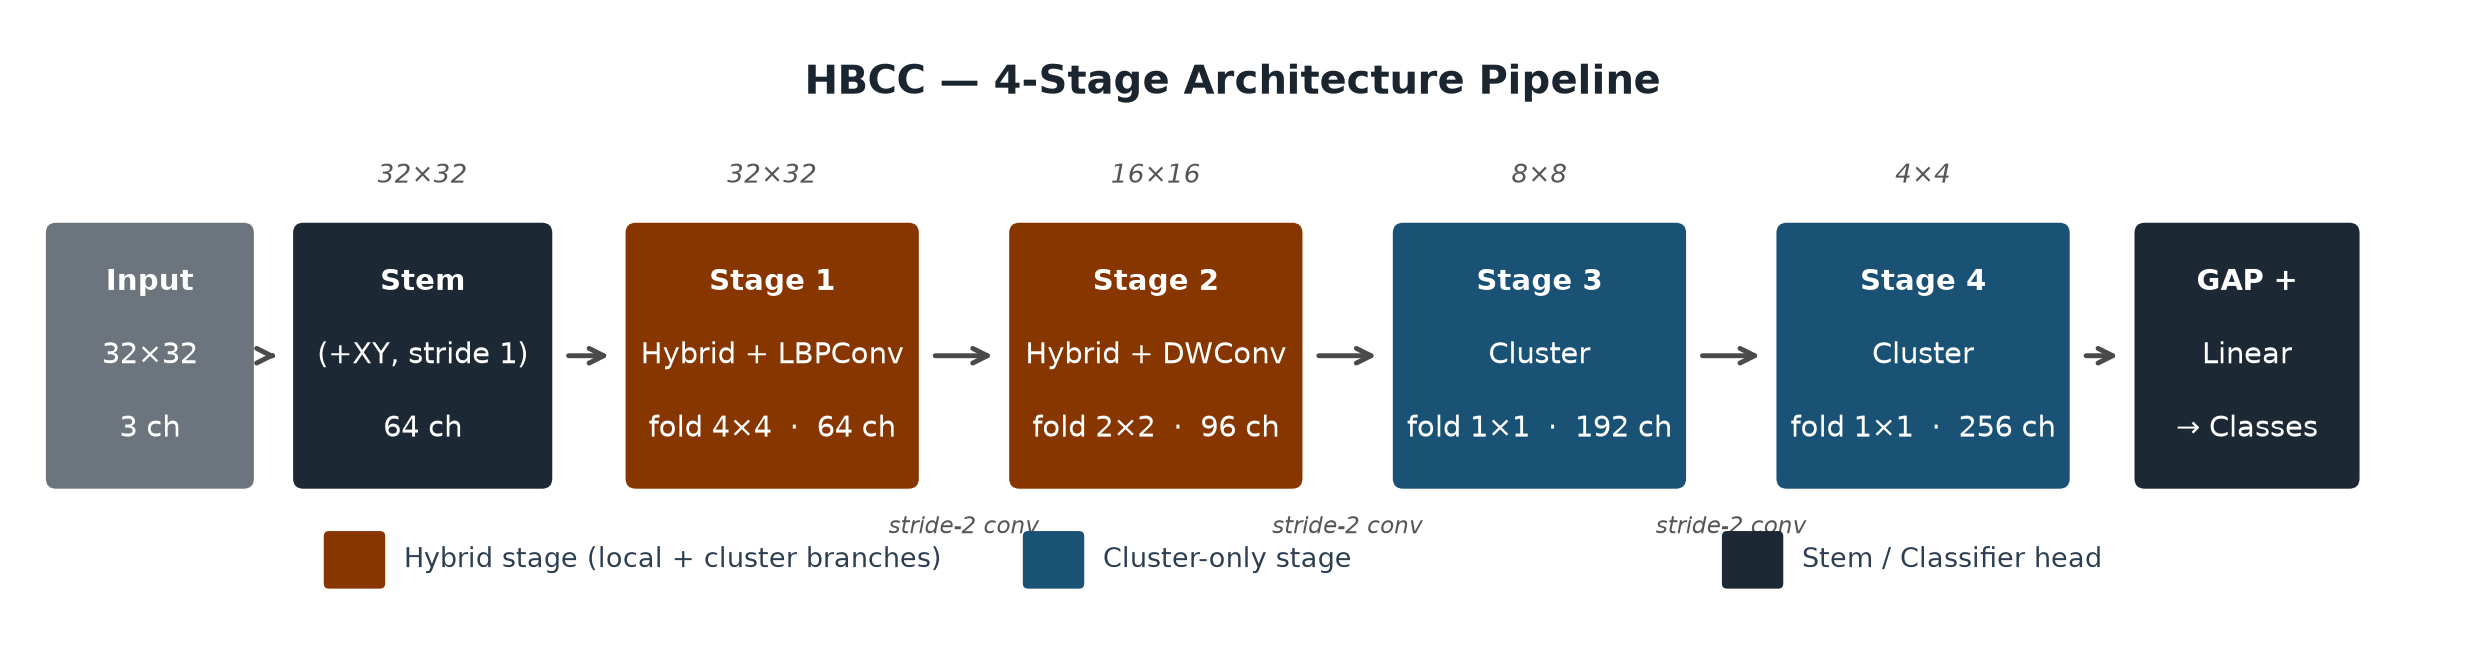
\includegraphics[width=0.96\textwidth]{fig_hbcc_pipeline}
  \end{center}

  \vspace{0.2em}
  \begin{itemize}\setlength\itemsep{5pt}
    \item \textbf{Stem} (stride = 1): RGB $32\!\times\!32$ $\to$
          $32\!\times\!32\!\times\!64$; spatial coordinates $(x,y)$
          are injected here.
    \item Resolution is halved between stages via a stride-2 conv.
    \item \textbf{GAP + Linear} classifier at the end.
  \end{itemize}
\end{frame}

% ============================================================
% Slide 10: Token Degeneracy
% ============================================================
\begin{frame}{Token Degeneracy: A Critical Design Fix}
  \begin{block}{Problem discovered during development}
    With \texttt{stem\_stride = 2}, Stage 4 clustering became a no-op.
  \end{block}

  \begin{columns}[T]
    \begin{column}{0.47\textwidth}
      \textbf{Root cause (stride = 2):}
      \begin{itemize}\small\setlength\itemsep{3pt}
        \item After stem: only $16\!\times\!16$ feature map.
        \item By Stage 4: $2\!\times\!2 = 4$ points remain.
        \item 4 cluster centers $\Rightarrow$ each cluster
              has \textbf{exactly 1 point}.
        \item Clustering is the identity function ---
              Stage 4 learns \textbf{nothing}.
      \end{itemize}
    \end{column}
    \begin{column}{0.50\textwidth}
      \textbf{Fix: set stem\_stride = 1}
      \begin{itemize}\small\setlength\itemsep{2pt}
        \item Stem output: $32\!\times\!32$ (4$\times$ more points).
        \item Every stage achieves $r = 16$ pts/cluster:
          \begin{itemize}\footnotesize\setlength\itemsep{2pt}
            \item Stages 1--3: 64 pts $\div$ 4 centers $= r\!=\!16$
            \item Stage 4: 16 pts $\div$ 1 center $= r\!=\!16$
          \end{itemize}
        \item Clustering meaningful at every stage. \checkmark
        \item Depth reduced $[2,2,4,2]\!\to\![1,1,2,1]$ to compensate.
      \end{itemize}
    \end{column}
  \end{columns}
\end{frame}

% ============================================================
% Slide 11: Knowledge Distillation
% ============================================================
\begin{frame}{Knowledge Distillation (KD)}
  \begin{block}{Goal}
    Boost HBCC accuracy from ResNet-18 teacher ---
    \textbf{no extra parameters at inference}.
  \end{block}

  \begin{columns}[T]
    \begin{column}{0.54\textwidth}
      \begin{itemize}\setlength\itemsep{5pt}
        \item \textbf{Teacher:} ResNet-18 (11M), trained from scratch\\
              on the same data (C-10: 96.48\%, C-100: 79.57\%).
        \item \textbf{Loss:} $\alpha{=}0.5$ mix of cross-entropy
              (hard labels) and KL-divergence (soft teacher logits).
        \item \textbf{Temperature} $T = 4$: softens logits to
              reveal inter-class similarity.
        \item Teacher is \textbf{frozen} during student training.
      \end{itemize}
    \end{column}
    \begin{column}{0.42\textwidth}
      \centering
      \vspace{0.2em}
      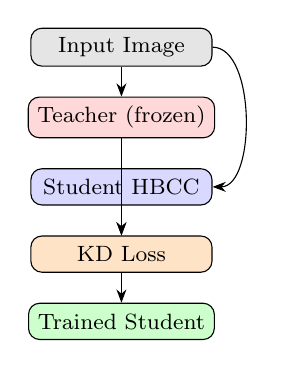
\begin{tikzpicture}[>=Stealth, node distance=0.38cm,
          every node/.style={font=\footnotesize, align=center},
          box/.style={draw, rounded corners, minimum width=2.3cm,
                      minimum height=0.46cm}]
        \node[box, fill=gray!20]             (img) {Input Image};
        \node[box, fill=red!15,  below=of img]  (tea) {Teacher (frozen)};
        \node[box, fill=blue!15, below=of tea]  (stu) {Student HBCC};
        \node[box, fill=orange!22,below=of stu] (kd)  {KD Loss};
        \node[box, fill=green!20, below=of kd]  (out) {Trained Student};
        \draw[->] (img) -- (tea);
        \draw[->] (img.east) to[out=0,in=0,looseness=0.8] (stu.east);
        \draw[->] (tea) -- (kd);
        \draw[->] (stu) -- (kd);
        \draw[->] (kd)  -- (out);
      \end{tikzpicture}
    \end{column}
  \end{columns}
\end{frame}

\section{Experiments \& Results}

% ============================================================
% Slide 12: Experimental Setup — Training
% ============================================================
\begin{frame}{Experimental Setup (1/2): Training Recipe}
  \begin{columns}[T]
    \begin{column}{0.48\textwidth}
      \textbf{Optimizer \& Schedule:}
      \begin{itemize}\setlength\itemsep{5pt}
        \item AdamW: lr $= 10^{-3}$, weight decay $= 0.05$.
        \item Cosine annealing, 5-epoch linear warmup.
        \item 300 epochs (CE) / 250 epochs (KD).
        \item Label smoothing $= 0.1$.
        \item Mixed precision (AMP / FP16).
        \item Drop path: 0.05 (Small), 0.08 (Medium).
      \end{itemize}
    \end{column}
    \begin{column}{0.48\textwidth}
      \textbf{Data Augmentation:}
      \begin{itemize}\setlength\itemsep{5pt}
        \item RandAugment ($N\!=\!2$, $M\!=\!9$).
        \item MixUp ($\alpha\!=\!0.2$).
        \item CutMix ($\alpha\!=\!1.0$, $p\!=\!0.5$).
        \item Random Erasing ($p\!=\!0.25$).
        \item Horizontal flip + random crop.
      \end{itemize}
    \end{column}
  \end{columns}
\end{frame}

% ============================================================
% Slide 13: Experimental Setup — Baselines & Evaluation
% ============================================================
\begin{frame}{Experimental Setup (2/2): Baselines \& Evaluation}
  \begin{columns}[T]
    \begin{column}{0.50\textwidth}
      \textbf{Baselines}\\
      {\small Standard augmentation, 300 epochs:}
      \begin{itemize}\setlength\itemsep{6pt}
        \item ResNet-18 --- upper-bound reference
              \& KD teacher.
        \item MobileNetV2.
        \item ShuffleNetV2-x1.0.
        \item CoC-baseline --- pure clustering,
              no local branch.
      \end{itemize}
    \end{column}
    \begin{column}{0.46\textwidth}
      \textbf{Evaluation Protocol:}
      \begin{itemize}\setlength\itemsep{6pt}
        \item Split: 45K train / 5K val / 10K test,
              seed 42 (fixed for all models).
        \item Test set used \textbf{once} only,
              for final reporting.
        \item \textbf{Latency:} Tesla T4 GPU,
              batch\,=\,1, 100 synchronized runs.
        \item \textbf{MACs \& Params:} \texttt{fvcore}
              (clustering ops may be undercounted).
      \end{itemize}
    \end{column}
  \end{columns}
\end{frame}

% ============================================================
% Slide 14: Results on CIFAR-10
% ============================================================
\begin{frame}{Results on CIFAR-10}
  \begin{block}{Highlight}
    HBCC-Med+KD: \textbf{95.36\%} --- 6.3$\times$ fewer params than ResNet-18.
    HBCC-Sml+KD (1.27M): \textbf{+3.25\%} over ShuffleNetV2 at the same budget.
    HBCC-Med+KD: \textbf{+7.02\%} over CoC-baseline and also faster.
  \end{block}

  \vspace{0.15em}
  \centering\small
  \begin{tabular}{lrrrr}
    \toprule
    \textbf{Model} & \textbf{Params} & \textbf{MACs}
      & \textbf{Latency} & \textbf{Top-1} \\
    \midrule
    ResNet-18              & 11.17M & 557M & 3.0\,ms  & 96.48\% \\
    \midrule
    ShuffleNetV2-x1.0      &  1.26M &  46M & 6.3\,ms  & 91.68\% \\
    MobileNetV2            &  2.24M &  26M & 4.8\,ms  & 91.04\% \\
    CoC-baseline           &  2.40M &  34M & 11.7\,ms & 88.34\% \\
    \midrule
    HBCC-Small (CE)        &  1.27M &  92M & 7.8\,ms  & 94.00\% \\
    HBCC-Medium (CE)       &  1.76M & 139M & 7.9\,ms  & 94.45\% \\
    HBCC-Small+KD          &  1.27M &  92M & 8.4\,ms  & 94.93\% \\
    \textbf{HBCC-Med+KD}   &\textbf{1.76M}&\textbf{139M}&\textbf{8.1\,ms}&\textbf{95.36\%}\\
    \bottomrule
  \end{tabular}
\end{frame}

% ============================================================
% Slide 15: Results on CIFAR-100
% ============================================================
\begin{frame}{Results on CIFAR-100}
  \begin{block}{Highlight}
    HBCC-Medium+KD: \textbf{77.68\%} --- best among lightweight models,
    1.89\% below ResNet-18.
    \textit{Without KD, HBCC falls below ShuffleNetV2 --- KD is decisive.}
  \end{block}

  \vspace{0.2em}
  \centering\small
  \begin{tabular}{lrrcc}
    \toprule
    \textbf{Model} & \textbf{Params} & \textbf{MACs}
      & \textbf{Top-1} & \textbf{Top-5} \\
    \midrule
    ResNet-18              & 11.22M & 557M & 79.57\% & 93.97\% \\
    \midrule
    ShuffleNetV2-x1.0      &  1.36M &  46M & 76.46\% & 93.43\% \\
    MobileNetV2            &  2.35M &  26M & 73.75\% & 92.54\% \\
    CoC-baseline           &  2.42M &  34M & 72.01\% & 90.70\% \\
    \midrule
    HBCC-Small (CE)        &  1.30M &  92M & 75.40\% & 92.93\% \\
    HBCC-Medium (CE)       &  1.78M & 139M & 75.59\% & 92.76\% \\
    HBCC-Small+KD          &  1.30M &  92M & 76.75\% & 93.95\% \\
    \textbf{HBCC-Med+KD}   &\textbf{1.78M}&\textbf{139M}&\textbf{77.68\%}&\textbf{93.86\%}\\
    \bottomrule
  \end{tabular}
\end{frame}

% ============================================================
% Slide 16: Pareto Analysis
% ============================================================
\begin{frame}{Pareto Analysis: Accuracy vs.\ Parameters \& Latency}
  \begin{columns}[T]
    \begin{column}{0.50\textwidth}
      \centering
      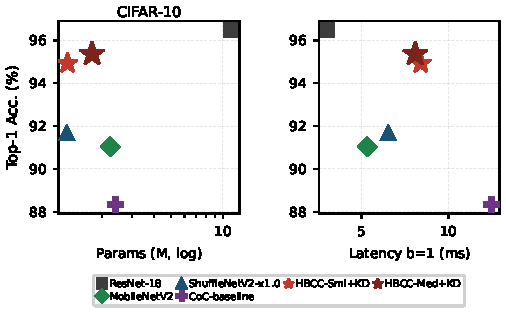
\includegraphics[width=\textwidth]{pareto_cifar10}\\
      {\footnotesize CIFAR-10}
    \end{column}
    \begin{column}{0.50\textwidth}
      \centering
      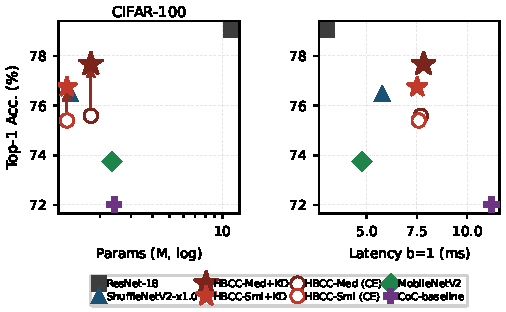
\includegraphics[width=\textwidth]{pareto_cifar100}\\
      {\footnotesize CIFAR-100}
    \end{column}
  \end{columns}

  \vspace{0.3em}
  \begin{itemize}
    \item \textbf{Stars ($\bigstar$):} HBCC+KD occupy the \textbf{upper-left}
          --- best accuracy at lowest parameter count.
  \end{itemize}
\end{frame}

\section{Limitations \& Conclusion}

% ============================================================
% Slide 17: Limitations
% ============================================================
\begin{frame}{Limitations}
  \begin{enumerate}\setlength\itemsep{9pt}
    \item \textbf{Training recipe asymmetry.}
          HBCC uses RandAugment, MixUp, and CutMix;
          baselines use standard augmentation.
          Part of the accuracy gap reflects augmentation, not architecture.

    \item \textbf{High inference latency.}
          Clustering ops (scatter, cosine sim, sigmoid) are not cuDNN-fused
          $\to$ GPU kernel overhead dominates.
          HBCC ($\sim$8\,ms) is slower than ShuffleNetV2 (6\,ms) at batch\,=\,1.

    \item \textbf{MACs undercount.}
          \texttt{fvcore} omits \texttt{scatter\_} and sigmoid inside
          clustering --- reported MACs are a lower bound.

    \item \textbf{CIFAR-only evaluation.}
          All experiments use $32\!\times\!32$ images.
          Generalization to ImageNet ($224\!\times\!224$) is unverified.
  \end{enumerate}
\end{frame}

% ============================================================
% Slide 18: Conclusion — Contributions
% ============================================================
\begin{frame}{Conclusion: Contributions}
  \begin{block}{Summary}
    Combining local operators with global clustering in a progressive
    4-stage design outperforms all lightweight baselines on CIFAR-10/100.
  \end{block}

  \vspace{0.5em}
  \textbf{Key Contributions:}
  \begin{enumerate}\setlength\itemsep{9pt}
    \item \textbf{Hybrid block:} channel-split local + CoC branches
          combined with layer-scale residuals and drop path.
    \item \textbf{Fold partitioning:} progressively widens CoC's
          receptive field from local (high-res) to global (low-res).
    \item \textbf{Token-degeneracy fix:} identified and resolved
          the bug where \texttt{stem\_stride = 2} made Stage 4 a no-op.
    \item \textbf{Knowledge Distillation:} response-based KD from
          ResNet-18 adds $+$0.9\% on CIFAR-10, $+$2.1\% on CIFAR-100.
  \end{enumerate}
\end{frame}

% ============================================================
% Slide 19: Conclusion — Results & Future Work
% ============================================================
\begin{frame}{Conclusion: Results \& Future Work}
  \begin{columns}[T]
    \begin{column}{0.50\textwidth}
      \begin{block}{Best Results}
        \begin{itemize}\setlength\itemsep{6pt}
          \item CIFAR-10: \textbf{95.36\%}\\
                (Med+KD, 1.76M params)
          \item CIFAR-100: \textbf{77.68\%}\\
                (Med+KD, 1.78M params)
          \item Pareto-dominant over all\\
                lightweight baselines on\\
                the parameter axis.
        \end{itemize}
      \end{block}
    \end{column}
    \begin{column}{0.46\textwidth}
      \begin{alertblock}{Future Work}
        \begin{itemize}\setlength\itemsep{6pt}
          \item Fused CUDA/Triton kernel
                for clustering ops to reduce
                inference latency.
          \item Scale experiments to
                \textbf{ImageNet-1K}.
          \item Feature-based KD
                (intermediate layers,
                not only logits).
        \end{itemize}
      \end{alertblock}
    \end{column}
  \end{columns}
\end{frame}

% ============================================================
% Slide 19: Q&A
% ============================================================
\begin{frame}{}
  \vspace{2.5em}
  \centering
  {\LARGE \textbf{Thank You}}

  \vspace{1.5em}
  {\large Questions \& Discussion}

  \vspace{2em}
  \begin{columns}
    \begin{column}{0.5\textwidth}
      \centering\small
      \textbf{Nguy\~{\^e}n Vi\d{\^e}t H\`ung}\\
      MSSV: 23122032
    \end{column}
    \begin{column}{0.5\textwidth}
      \centering\small
      \textbf{Nguy\~{\^e}n B\'a Nam}\\
      MSSV: 23122043
    \end{column}
  \end{columns}
\end{frame}

\end{document}